\documentclass[11pt]{article}
\usepackage[margin=1in]{geometry}
\usepackage[T1]{fontenc}
\usepackage{amsmath,amssymb,booktabs,graphicx}
\usepackage[round]{natbib}
\usepackage[hidelinks]{hyperref}
\usepackage{pgf}
% \ppd{precision}{expression}: decimal result computed from the macros by pgfmath (no typed result).
\newcommand{\ppd}[2]{\pgfmathparse{#2}\pgfmathprintnumber[fixed,precision=#1]{\pgfmathresult}}

% Result numbers. Generated by `crew.py numbers`; never typed by hand.
% Generated by `crew.py numbers` from claims.jsonl. Do not edit by hand.
% Each macro is a number taken from a logged run; see claims.jsonl.
\newcommand{\RdEffect}{7.416}  % rd-effect
\newcommand{\RdCiLow}{4.094}  % rd-ci-low
\newcommand{\RdCiHigh}{10.925}  % rd-ci-high
\newcommand{\RdSe}{1.460}  % rd-conv-se
\newcommand{\RdRobustSe}{1.743}  % rd-robust-se
\newcommand{\RdN}{1,297}  % rd-n
\newcommand{\RdNLeft}{595}  % rd-n-left
\newcommand{\RdNRight}{702}  % rd-n-right
\newcommand{\RdBw}{17.708}  % rd-bw
\newcommand{\RdB}{27.984}  % rd-b
\newcommand{\RdDistinctRight}{665}  % rd-distinct-right
\newcommand{\RdMassRight}{0.053}  % rd-mass-share-right
\newcommand{\RdAdjEffect}{7.414}  % rd-adj-effect
\newcommand{\RdAdjCiLow}{4.094}  % rd-adj-ci-low
\newcommand{\RdAdjCiHigh}{10.919}  % rd-adj-ci-high
\newcommand{\RdAdjBw}{17.754}  % rd-adj-bw
\newcommand{\RdDensityP}{0.381}  % rd-density-p
\newcommand{\RdDensityT}{-0.875}  % rd-density-t
\newcommand{\RdDensityPConv}{0.099}  % rd-density-p-conv
\newcommand{\RdDensityPNomass}{0.381}  % rd-density-p-nomass
\newcommand{\RdDensityDiff}{-0.0035}  % rd-density-diff
\newcommand{\RdCovClassP}{0.897}  % rd-cov-class-p
\newcommand{\RdCovClassHolm}{1.000}  % rd-cov-class-holm
\newcommand{\RdCovClassMde}{0.401}  % rd-cov-class-mde
\newcommand{\RdCovClassCoef}{-0.021}  % rd-cov-class-coef
\newcommand{\RdCovClassN}{1,390}  % rd-cov-class-n
\newcommand{\RdCovClassOffMinusPrinted}{0.0003}  % rd-cov-class-printed-off
\newcommand{\RdCovClassAdjP}{0.896}  % rd-cov-class-adj-p
\newcommand{\RdCovTermshouseP}{0.561}  % rd-cov-termshouse-p
\newcommand{\RdCovTermshouseHolm}{1.000}  % rd-cov-termshouse-holm
\newcommand{\RdCovTermshouseMde}{1.400}  % rd-cov-termshouse-mde
\newcommand{\RdCovTermshouseCoef}{-0.173}  % rd-cov-termshouse-coef
\newcommand{\RdCovTermshouseN}{1,108}  % rd-cov-termshouse-n
\newcommand{\RdCovTermshouseOffMinusPrinted}{0.0002}  % rd-cov-termshouse-printed-off
\newcommand{\RdCovTermshouseAdjP}{0.561}  % rd-cov-termshouse-adj-p
\newcommand{\RdCovTermssenateP}{0.901}  % rd-cov-termssenate-p
\newcommand{\RdCovTermssenateHolm}{1.000}  % rd-cov-termssenate-holm
\newcommand{\RdCovTermssenateMde}{2.091}  % rd-cov-termssenate-mde
\newcommand{\RdCovTermssenateCoef}{-0.192}  % rd-cov-termssenate-coef
\newcommand{\RdCovTermssenateN}{1,108}  % rd-cov-termssenate-n
\newcommand{\RdCovTermssenateOffMinusPrinted}{-0.0002}  % rd-cov-termssenate-printed-off
\newcommand{\RdCovTermssenateAdjP}{0.900}  % rd-cov-termssenate-adj-p
\newcommand{\RdCovPopulationP}{0.634}  % rd-cov-population-p
\newcommand{\RdCovPopulationHolm}{1.000}  % rd-cov-population-holm
\newcommand{\RdCovPopulationMde}{2,185,253}  % rd-cov-population-mde
\newcommand{\RdCovPopulationCoef}{-318,455}  % rd-cov-population-coef
\newcommand{\RdCovPopulationN}{1,390}  % rd-cov-population-n
\newcommand{\RdCovPopulationOffMinusPrinted}{0.0002}  % rd-cov-population-printed-off
\newcommand{\RdCovPopulationAdjP}{0.634}  % rd-cov-population-adj-p
\newcommand{\RdPlaceboCL}{-14.345}  % rd-placebo-cl
\newcommand{\RdPlaceboCR}{20.440}  % rd-placebo-cr
\newcommand{\RdPlaceboLeftEst}{-0.029}  % rd-placebo-left-est
\newcommand{\RdPlaceboLeftCiLow}{-12.168}  % rd-placebo-left-ci-low
\newcommand{\RdPlaceboLeftCiHigh}{14.141}  % rd-placebo-left-ci-high
\newcommand{\RdPlaceboLeftN}{595}  % rd-placebo-left-n
\newcommand{\RdPlaceboLeftCapped}{0}  % rd-placebo-left-capped
\newcommand{\RdPlaceboRightEst}{-1.068}  % rd-placebo-right-est
\newcommand{\RdPlaceboRightCiLow}{-11.287}  % rd-placebo-right-ci-low
\newcommand{\RdPlaceboRightCiHigh}{11.274}  % rd-placebo-right-ci-high
\newcommand{\RdPlaceboRightN}{702}  % rd-placebo-right-n
\newcommand{\RdPlaceboRightCapped}{0}  % rd-placebo-right-capped
\newcommand{\RdSelectionP}{0.125}  % rd-selection-p
\newcommand{\RdSelectionCoef}{-0.062}  % rd-selection-coef
\newcommand{\RdSelectionMde}{11.6}  % rd-selection-mde
\newcommand{\RdSelectionObserved}{0.933}  % rd-selection-observed
\newcommand{\RdSensPrintedEst}{7.425}  % rd-h3-h3-2014-bw-effect
\newcommand{\RdSensPrintedLo}{4.070}  % rd-h3-h3-2014-bw-ci-low
\newcommand{\RdSensPrintedHi}{10.983}  % rd-h3-h3-2014-bw-ci-high
\newcommand{\RdSensPrintedBw}{16.794}  % rd-h3-h3-2014-bw-bw
\newcommand{\RdSensPrintedB}{27.437}  % rd-h3-h3-2014-bw-b
\newcommand{\RdSensPrintedN}{1,297}  % rd-h3-h3-2014-bw-n
\newcommand{\RdSensHalfEst}{8.373}  % rd-h3-half-bw-effect
\newcommand{\RdSensHalfLo}{4.756}  % rd-h3-half-bw-ci-low
\newcommand{\RdSensHalfHi}{14.031}  % rd-h3-half-bw-ci-high
\newcommand{\RdSensHalfBw}{8.854}  % rd-h3-half-bw-bw
\newcommand{\RdSensHalfB}{13.992}  % rd-h3-half-bw-b
\newcommand{\RdSensHalfN}{1,297}  % rd-h3-half-bw-n
\newcommand{\RdSensDoubleEst}{7.168}  % rd-h3-double-bw-effect
\newcommand{\RdSensDoubleLo}{5.358}  % rd-h3-double-bw-ci-low
\newcommand{\RdSensDoubleHi}{10.646}  % rd-h3-double-bw-ci-high
\newcommand{\RdSensDoubleBw}{35.416}  % rd-h3-double-bw-bw
\newcommand{\RdSensDoubleB}{55.968}  % rd-h3-double-bw-b
\newcommand{\RdSensDoubleN}{1,297}  % rd-h3-double-bw-n
\newcommand{\RdSensPTwoEst}{8.046}  % rd-h3-p2-effect
\newcommand{\RdSensPTwoLo}{4.213}  % rd-h3-p2-ci-low
\newcommand{\RdSensPTwoHi}{12.423}  % rd-h3-p2-ci-high
\newcommand{\RdSensPTwoBw}{22.210}  % rd-h3-p2-bw
\newcommand{\RdSensPTwoB}{33.245}  % rd-h3-p2-b
\newcommand{\RdSensPTwoN}{1,297}  % rd-h3-p2-n
\newcommand{\RdSensAdjustEst}{7.414}  % rd-h3-adjust-effect
\newcommand{\RdSensAdjustLo}{4.094}  % rd-h3-adjust-ci-low
\newcommand{\RdSensAdjustHi}{10.919}  % rd-h3-adjust-ci-high
\newcommand{\RdSensAdjustBw}{17.754}  % rd-h3-adjust-bw
\newcommand{\RdSensAdjustB}{28.028}  % rd-h3-adjust-b
\newcommand{\RdSensAdjustN}{1,297}  % rd-h3-adjust-n


% Allow slightly loose lines instead of overfull boxes in long \texttt names.
\emergencystretch=3em

\title{The Local Effect of a Democratic Senate Win in Close Races:\\
A Regression-Discontinuity Replication with a Pinned Pipeline and Falsification Checks}
\author{Bryce Wang \\ \small Drafted with Free-Research-Crew; see the AI-use statement.}
\date{\today}

\begin{document}
\maketitle

\begin{abstract}
We replicate the default regression-discontinuity output that \citet{calonico2017rdrobust} print for the effect of a Democratic US Senate win on the Democratic vote share in the next election for the same seat. We use the public 1914--2010 file distributed with the rdrobust package, a pinned software version, and a tolerance fixed before the run. The conventional local-linear estimate is \RdEffect\ percentage points, with a robust bias-corrected 95\% confidence interval of $[\RdCiLow, \RdCiHigh]$ on \RdN\ elections. This holds under \texttt{masspoints = off}, an unverified assumption that the Designer chose knowing the printed targets. Under the software default, \texttt{adjust}, the bandwidth is \RdAdjBw\ against a printed 17.708 and misses the tolerance, and two covariate p-values also miss their printed values. It is a computational check and makes no new claim about the incumbency advantage, and the estimate is local to close elections. Falsification tests were fixed before the outcome analysis. The density statistic and the covariate standard errors and MDEs were computed before the design gate, from margin and covariates only. The density, covariate and selection tests do not reject at conventional levels, but they are imprecise, and the selection test's interval is wide. The placebo cutoffs are reported without a test. Across five descriptive sensitivity specifications, the point estimate ranges from \RdSensDoubleEst\ to \RdSensHalfEst\ percentage points.
\end{abstract}

\section{Introduction}

In close US Senate elections, does a Democratic win make the Democratic party more likely to win the same seat six years later? \citet{calonico2017rdrobust} use this question to illustrate the default output of the rdrobust software. Their Section 7.2 prints the conventional local-linear estimate, its robust bias-corrected confidence interval and the bandwidths, for the Senate data analysed by \citet{cattaneo2015randomization}. The case is a useful test of reproducibility. The data are public, the design is standard, and the same file has been analysed with other RD methods \citep{cattaneo2016rdlocrand}.

This paper is a replication. It claims no new finding about the incumbency advantage. Here the phrase is the literature's label for the effect of a win on the same party's later win. The treatment is a Democratic win by whichever candidate, not a win by an incumbent, so the estimand is a party advantage in close races, and the phrase is used only in that sense. It has three aims: (i) to reproduce the printed default output with a pinned software version, a tolerance fixed before the run, and a logged pipeline; (ii) to report a set of falsification checks whose tests, samples and minimum detectable effects were fixed before any outcome analysis; and (iii) to show how far the estimate and the checks move across the bandwidth and software choices that the printed output leaves open.

In brief, the printed default output is reproduced within the tolerance set in advance under \texttt{masspoints = off}, an unverified assumption that the Designer chose knowing the printed targets. Under the software default, \texttt{adjust}, the bandwidth misses the tolerance and two covariate p-values miss their printed values. The conventional estimate is \RdEffect\ percentage points, the robust interval is $[\RdCiLow, \RdCiHigh]$, and the sample is \RdN\ elections. This is a computational check. A deterministic package at a fixed version should reproduce its own output, so the match shows that the pipeline works and says little about the world. The falsification checks do not reject at conventional levels. They are, however, imprecise: their minimum detectable effects are large relative to the quantities they test, and the selection test's interval is wide. Across the five descriptive sensitivity specifications, the point estimate lies between \RdSensDoubleEst\ and \RdSensHalfEst\ percentage points, and every interval overlaps the main one.

Section 2 describes the data. Section 3 sets out the estimand, the estimator and the planned checks. Section 4 reports the results. Section 5 gives the limitations, and Section 6 lists every deviation from the approved design and every disclosure. Section 7 concludes.

\section{Data}

The data are \texttt{rdrobust\_senate.csv} from the rdrobust repository (commit 2589686d). The file has one row per US Senate election, 1914 to 2010, across 50 states, for \RdDensityN\ rows in total. The running variable \texttt{margin} is the Democratic margin of victory at election $t$, in percentage points, with the cutoff at 0. Of the rows, \RdDensityNLeft\ have a negative margin and \RdDensityNRight\ have a margin at or above 0. The outcome \texttt{vote} is the Democratic vote share, in percent, in the next election for the same seat ($t+2$). Missing outcomes are dropped by the estimator, which leaves \RdN\ elections with an observed outcome (\RdNLeft\ below the cutoff and \RdNRight\ at or above it).

The file contains four predetermined covariates: \texttt{class}, \texttt{termshouse}, \texttt{termssenate} and \texttt{population}. Two of them, \texttt{termshouse} and \texttt{termssenate}, are missing on the same rows, so their balance tests use \RdCovTermshouseN\ elections. The file has four of the eight predetermined covariates that \citet{cattaneo2015randomization} use. The balance tests here are therefore not the tests of that paper.

The printed output of \citet{calonico2017rdrobust} comes from the Stata implementation of the 2016 release. The file used here is the CSV in the rdrobust repository, not the \texttt{.dta} file the authors used. Before the H1 run, the design-stage checks compared the printed descriptive statistics for the non-outcome variables with the file, at printed precision, and found agreement. The moments of \texttt{vote} were not compared with any source before the H1 run, so the fidelity of the outcome is established only by the H1 comparison itself. Margin is tied only at $\pm 100$. In the H1 sample, the left side has \RdDistinctLeft\ distinct margin values for \RdNLeft\ elections, so it has no repeats. The right side has \RdDistinctRight\ distinct values for \RdNRight\ elections. The tied observations all sit at +100, and the share of right-side observations that repeat an earlier margin value is \RdMassRight\ (counting only the repeats beyond the first at each value). No tie lies within 30 points of the cutoff. The raw file is not committed to the repository. Its SHA-256 hash is recorded in the manifest.

\section{Empirical strategy}

\subsection{Estimand and identifying assumption}

The estimand is the effect of a Democratic win on the Democratic vote share in the next election for the same seat, identified at the cutoff. The comparison is between seats where the Democrats won narrowly and seats where they lost narrowly. The estimate is local: it describes close elections, not all elections. The identifying assumption, in plain words, is that the expected next-election vote share would change smoothly through the cutoff if the Democrats had not won. This would fail if candidates could precisely manipulate the margin, or if other determinants of the outcome jumped at the cutoff. Both are checked below, but neither check can prove the assumption.

\subsection{Estimator and settings}

The estimator is a sharp RD with a local-linear fit. For each side $s$ of the cutoff, the intercept $\alpha_s$ and slope $\beta_s$ solve a weighted least-squares problem on the elections within the bandwidth $h$:
\begin{equation}
(\hat\alpha_s,\hat\beta_s)=\arg\min_{a,b}\sum_{i:\,s(M_i)}K\!\left(\frac{M_i}{h}\right)\bigl(Y_i-a-bM_i\bigr)^2,
\qquad
\hat\tau=\hat\alpha_{+}-\hat\alpha_{-},
\end{equation}
where $M_i$ is the margin, $Y_i$ the vote share, $K(u)=(1-|u|)_+$ the triangular kernel, and $s(M_i)$ selects $M_i\ge 0$ on the right and $M_i<0$ on the left. The settings are those of the printed default output: polynomial order $p=1$, bias-correction order $q=2$, the triangular kernel, the MSE-optimal common bandwidth (\texttt{mserd}), nearest-neighbour variance with three matches, and a robust bias-corrected 95\% interval. No covariates enter the H1 specification.

\subsection{Software and the \texttt{masspoints} setting}

The software is the Python rdrobust package, version 2.1.1, and the rddensity package, version 3.0, both pinned in the code requirements. The printed output comes from the 2016 Stata release, so the implementation and version differ from those used here.

The rdrobust 2.1.1 bandwidth selector has an option, \texttt{masspoints}, that changes how repeated margin values enter the selector. Its default is \texttt{adjust}. The printed output was produced by an earlier release, and we have not verified whether that release used no mass-point adjustment. We therefore treat \texttt{off} as the primary setting, on the assumption that the 2016 release used no adjustment, and report \texttt{adjust} alongside it. This assumption is not verified; no source in the workspace documents the earlier release's default. The Designer chose \texttt{off} at the design stage knowing the printed targets, and the H1 targets were named in the plan before the run. The printed bandwidths agree with \texttt{off} (17.708 within the tolerance; the bias bandwidth is \RdBOff\ against the printed 27.984, which is not a tolerance target) and not with \texttt{adjust} (\ppd{3}{\RdAdjBw} and \ppd{3}{\RdBAdj}). That agreement is consistent with the assumption. It is not independent evidence for it, because the choice and the targets were both known at design, and the H1 pass is conditional on that choice.

\subsection{Tolerances and planned checks}

Before the H1 run, the tolerance rule was fixed. The replicated conventional estimate must lie within 0.01 percentage points of 7.416. Each endpoint of the robust interval must lie within 0.01 percentage points of its printed value, $[4.09441, 10.9255]$. The sample size must match exactly, with $N=1{,}297$. The bandwidth must lie within 0.0005 of the printed value of 17.708. The decision is made on the \texttt{off} setting only. A failure would be reported as a failure, diagnosed by version, platform or option, and not replaced by the other setting.

The falsification checks were fixed at the design gate, with the exceptions stated below, and are reported without a conclusion drawn across the families of tests:
\begin{description}
\item[H2(a)] A density test of margin at 0, using rddensity on all \RdDensityN\ margins with the robust bias-corrected statistic as primary. The minimum detectable difference (MDE) is the difference that would be detected with 80\% power at a two-sided 5\% level.
\item[H2(b)] Balance of the four covariates at the cutoff, each estimated with the H1 settings and \texttt{off}. The four robust p-values are Holm-adjusted together, and nothing else is corrected.
\item[H2(c)] One-sided placebo cutoffs at the median margin on each side of 0 (medians over all margins, with no outcome used), each estimated only on its own side. These are reported only: the estimate, interval, sample and bandwidth, with the interval width as the precision statement. No test and no conclusion are drawn.
\item[H2(d)] A test that the observed-outcome indicator (1 if the vote is non-missing) has no discontinuity at the cutoff. Its MDE is fixed in the design and computed after the gate.
\end{description}
H3 is a descriptive sensitivity analysis with no decision rule. It reports the H1 estimate under the printed 2014 bandwidths, under half and double the H1 bandwidth, with $p=2$ and $q=3$, and with \texttt{adjust}.

Non-rejection in H2(a), H2(b) and H2(d) is read only as no evidence of a discontinuity larger than the MDE in the same row. It is not proof of continuity or of no selection.

Two computations came before the design gate. Run \texttt{design-mde}, a data-prep run that loaded only margin and the covariates, computed the robust density statistic on margin (the H2(a) statistic), the density-difference estimate, its jackknife standard error and the density MDE (\RdDensityMde), and the covariate standard errors that give the H2(b) MDEs. The analysis runs repeated these with the same settings and reproduced them. The H2(d) MDE was computed after the gate. Section 6 gives the details.

\section{Results}

\subsection{Replication of the default output (H1)}

Table~\ref{tab:main} sets the replicated values beside the printed ones. Under the primary \texttt{off} setting, all tolerance checks pass. The conventional estimate is \RdEffect\ percentage points, against a printed 7.416. The robust interval is $[\RdCiLow, \RdCiHigh]$, against a printed $[4.09441, 10.9255]$. The sample is \RdN\ elections, the printed value. The bandwidth is \RdBw\ points, against a printed 17.708. The conventional standard error is \RdSe\ and the robust standard error is \RdRobustSe. The bias bandwidth $b$, which is not part of the tolerance rule, is \RdB, against a printed 27.984.

The \texttt{adjust} reading in the same run gives a conventional estimate of \RdAdjEffect\ and a robust interval of $[\RdAdjCiLow, \RdAdjCiHigh]$. Its bandwidth of \RdAdjBw\ misses the printed 17.708 by more than the 0.0005 tolerance, so it is not judged to reproduce the printed output. The difference lies in the bandwidth selector, which uses the number of distinct margin values in place of the sample size. Here that count is \RdAdjMLeft\ on the left and \RdAdjMRight\ on the right, \RdDistinctTotal\ in total, against \RdN\ observations. The bandwidth-check trigger of rdrobust 2.1.1 (a mass share of at least 20 percent on one side) is not reached on either side. So the two settings differ only in that selector input. Because the printed bandwidths are the output of the earlier release, they discriminate between the settings only as evidence. The \texttt{off} setting reproduces them, and the \texttt{adjust} setting does not. That agreement is consistent with the \texttt{off} assumption. It is not independent evidence for it, since the Designer chose \texttt{off} knowing the targets, and the H1 pass is conditional on that choice.

\begin{table}[t]
\centering
\caption{Replication of the default output of \citet{calonico2017rdrobust}, Section 7.2 (H1).}
\label{tab:main}
\resizebox{\textwidth}{!}{\begin{tabular}{lrrr}
\toprule
& Printed (CCFT 2017) & Replicated, \texttt{off} (primary) & Replicated, \texttt{adjust} (secondary) \\
\midrule
Conventional estimate (pp) & 7.416 & \RdEffect & \RdAdjEffect \\
Robust bias-corrected 95\% CI, lower (pp) & 4.09441 & \RdCiLow & \RdAdjCiLow \\
Robust bias-corrected 95\% CI, upper (pp) & 10.9255 & \RdCiHigh & \RdAdjCiHigh \\
$N$ (elections with an observed outcome) & 1,297 & \RdN & \RdSensAdjustN \\
Bandwidth $h$ (pp, both sides) & 17.708 & \RdBw & \RdAdjBw \\
Bias bandwidth $b$ (pp, left side) & 27.984 & \RdB & \RdSensAdjustB \\
\midrule
Tolerance check (estimate and CI within 0.01 pp; $N$ exact; $h$ within 0.0005) & -- & pass & not judged \\
\bottomrule
\end{tabular}
}
\par\smallskip
\footnotesize
\textit{Notes.} Specification: sharp RD; local-linear fit ($p=1$, $q=2$); triangular kernel; MSE-optimal common bandwidth; nearest-neighbour variance with three matches; robust bias-corrected 95\% interval. Outcome: Democratic vote share at $t+2$ in percent. Running variable: Democratic margin at $t$ in percentage points, cutoff 0. The printed column is the value stated in the article. The replicated columns use rdrobust 2.1.1. Intervals and estimates are in percentage points; the bias bandwidth $b$ is in margin points on the left side. The two replicated columns differ only in the \texttt{masspoints} option. The tolerance rule judges \texttt{off} only. The \texttt{adjust} column is secondary and is not judged.
\end{table}

These checks show that the pipeline reproduces the printed default output. They do not show anything about the incumbency advantage, because a deterministic package at a fixed version reproduces its own output.

\paragraph{Scope of the estimate.}
The H1 estimate is local to close elections. It uses elections within about \RdBw\ points of the cutoff, and it is conditional on the Democratic win at the threshold. It is the effect of a narrow Democratic win in close races. It is not the incumbency advantage in all elections, and the paper does not claim that it is.

\subsection{Falsification tests (H2)}

Table~\ref{tab:fals} reports each test with its own sample and MDE. Figure~\ref{fig:rd} shows the RD plot of the H1 sample, and Figure~\ref{fig:density} shows the density test.

\paragraph{Density (H2(a)).}
The robust bias-corrected test of equal densities at 0 gives $T_Q=\RdDensityT$ and a robust p-value of \RdDensityP. The conventional p-value from the same data is \RdDensityPConv, and it is not used for the decision. The robust p-value is primary, as fixed at the design gate, and the decision uses it; the conventional p-value is shown beside it in the same sentence for completeness. Neither is the McCrary test of \citet{cattaneo2015randomization}, whose p-value of 0.39 comes from their footnote 13 and is not the statistic reported here. The estimated density difference, right minus left, is \RdDensityDiff\ in density units, and its MDE is \RdDensityMde. With \texttt{massPoints = False} the robust p-value is \RdDensityPNomass, identical to the main value at full precision. The repeated margin values sit at $\pm 100$, outside both density bandwidths, and the kernel weights there are zero, so rddensity's mass-point adjustment has no observations inside the estimation window to act on. This follows from the code path (the jackknife branch of rddensity's variance function); it was not tested separately. Non-rejection here is read only as no evidence of a discontinuity larger than the MDE. It is not proof of continuity, and smaller discontinuities are not excluded.

\paragraph{Covariate balance (H2(b)).}
The four covariate tests are in Table~\ref{tab:fals}. None rejects. The Holm-adjusted p-values are \RdCovClassHolm, \RdCovTermshouseHolm, \RdCovTermssenateHolm\ and \RdCovPopulationHolm, in that order. The MDEs are large relative to the coefficients. For example, the class coefficient is \RdCovClassCoef\ against an MDE of \RdCovClassMde\ covariate units, and the population coefficient is \RdCovPopulationCoef\ persons against an MDE of \RdCovPopulationMde. The robust p-values under \texttt{off} are \RdCovClassP, \RdCovTermshouseP, \RdCovTermssenateP\ and \RdCovPopulationP. These agree with the printed values of 0.897, 0.561, 0.901 and 0.634 in \citet[p.~397]{calonico2017rdrobust}, within 0.0005 (half a unit in the printed third decimal), for all four under \texttt{off}. Under \texttt{adjust}, the robust p-values are \RdCovClassAdjP\ for class and \RdCovTermssenateAdjP\ for termssenate. Those two miss the printed values by more than 0.0005, while termshouse and population agree. The comparison with \texttt{off} is primary, as set in the plan's disclosures, and \texttt{adjust} is reported as secondary. Which masspoints setting the 2016 release used is unverified, so the paper does not establish which setting the printed values reflect. The agreement with \texttt{off} is consistent with the H1 assumption but does not verify it. The covariate tests use four of the eight covariates of \citet{cattaneo2015randomization}.

\paragraph{One-sided placebo cutoffs (H2(c)).}
The placebo cutoffs are $c_L=\RdPlaceboCL$ and $c_R=\RdPlaceboCR$, the medians of margin on each side of 0, taken over all \RdDensityN\ margins with no outcome used. Each placebo is estimated on its own side only, using the elections with an observed outcome there. The left placebo estimate is \RdPlaceboLeftEst, with a robust interval of $[\RdPlaceboLeftCiLow, \RdPlaceboLeftCiHigh]$ on \RdPlaceboLeftN\ elections. Its interval is \RdPlaceboLeftCiwidth\ points wide, and its bandwidth is \RdPlaceboLeftBw. The right placebo estimate is \RdPlaceboRightEst, with an interval of $[\RdPlaceboRightCiLow, \RdPlaceboRightCiHigh]$ on \RdPlaceboRightN\ elections, a width of \RdPlaceboRightCiwidth\ points, and a bandwidth of \RdPlaceboRightBw. The rdrobust bandwidth cap for the one-sided sample is \RdPlaceboLeftBwmax\ on the left and \RdPlaceboRightBwmax\ on the right. The recorded cap flag is \RdPlaceboLeftCapped\ on the left and \RdPlaceboRightCapped\ on the right. The reported bandwidths lie far below the caps, and the recorded flag agrees. The bias bandwidths recorded in the run are also far below the caps. The positive branch of the flag was tested only on forced inputs and never observed on output; it matters only if the code's cap formula differs from rdrobust's internal one. The effective samples within the bandwidth are small: \RdPlaceboLeftNhLeft\ and \RdPlaceboLeftNhRight\ elections on the two sides of $c_L$, and \RdPlaceboRightNhLeft\ and \RdPlaceboRightNhRight\ on the two sides of $c_R$. The placebo intervals are wide, and no conclusion is drawn from them.

\paragraph{Observed-outcome selection (H2(d)).}
The test is on the share of elections with an observed outcome, not on the vote. Its estimate is \RdSelectionCoef\ on the proportion scale (right minus left), which is \ppd{1}{100*(\RdSelectionCoef)} percentage points of that share. The robust interval is $[\RdSelectionCiLow, \RdSelectionCiHigh]$ on the same scale, which is $[\ppd{1}{100*(\RdSelectionCiLow)}, \ppd{1}{100*(\RdSelectionCiHigh)}]$ percentage points, and the p-value is \RdSelectionP. The single-test MDE is \RdSelectionMde\ percentage points. The point estimate is more than 80 percent of the H1 estimate of \RdEffect\ percentage points, as a size comparison only. That compares two quantities that measure different things, a change in the share of observed outcomes and a change in the vote share, so it is a comparison of size and not a bias calculation. This paper gives no mapping from a change in the observed-outcome share to a bias in the vote estimate, and no mechanism or bound links missing outcomes to the H1 estimate. The interval is wide, and the test is inconclusive. H1 is therefore not described as free of selection.

\begin{table}[t]
\centering
\caption{Falsification tests (H2) and descriptive sensitivity (H3).}
\label{tab:fals}
\resizebox{\textwidth}{!}{\begin{tabular}{lrrrr}
\toprule
Test (scale of estimate) & Estimate & 95\% CI or $p$ & $N$ & MDE (80\% power) \\
\midrule
\multicolumn{5}{l}{\emph{Panel A. Falsification tests (H2), each tested on its own}} \\
H2(a) density of margin at 0 (density units) & \RdDensityDiff & $p$ = \RdDensityP & \RdDensityN & \RdDensityMde \\
H2(b) class (covariate units) & \RdCovClassCoef & $p$ = \RdCovClassP (Holm \RdCovClassHolm) & \RdCovClassN & \RdCovClassMde \\
H2(b) termshouse (covariate units) & \RdCovTermshouseCoef & $p$ = \RdCovTermshouseP (Holm \RdCovTermshouseHolm) & \RdCovTermshouseN & \RdCovTermshouseMde \\
H2(b) termssenate (covariate units) & \RdCovTermssenateCoef & $p$ = \RdCovTermssenateP (Holm \RdCovTermssenateHolm) & \RdCovTermssenateN & \RdCovTermssenateMde \\
H2(b) population (persons) & \RdCovPopulationCoef & $p$ = \RdCovPopulationP (Holm \RdCovPopulationHolm) & \RdCovPopulationN & \RdCovPopulationMde \\
H2(c) placebo, left, $c_L$ = \RdPlaceboCL (report only; pp) & \RdPlaceboLeftEst & [\RdPlaceboLeftCiLow, \RdPlaceboLeftCiHigh] & \RdPlaceboLeftN & -- \\
H2(c) placebo, right, $c_R$ = \RdPlaceboCR (report only; pp) & \RdPlaceboRightEst & [\RdPlaceboRightCiLow, \RdPlaceboRightCiHigh] & \RdPlaceboRightN & -- \\
H2(d) observed-outcome share (proportion; MDE in pp) & \RdSelectionCoef & [\RdSelectionCiLow, \RdSelectionCiHigh]; $p$ = \RdSelectionP & \RdSelectionN & \RdSelectionMde \\
\midrule
\multicolumn{5}{l}{\emph{Panel B. H3 descriptive sensitivity of H1 (pp; no decision rule)}} \\
(i) printed 2014 bandwidths, $h$ = \RdSensPrintedBw & \RdSensPrintedEst & [\RdSensPrintedLo, \RdSensPrintedHi] & \RdSensPrintedN & -- \\
(ii) half H1 bandwidth, $h$ = \RdSensHalfBw & \RdSensHalfEst & [\RdSensHalfLo, \RdSensHalfHi] & \RdSensHalfN & -- \\
(iii) double H1 bandwidth, $h$ = \RdSensDoubleBw & \RdSensDoubleEst & [\RdSensDoubleLo, \RdSensDoubleHi] & \RdSensDoubleN & -- \\
(iv) $p$ = 2, $q$ = 3, $h$ = \RdSensPTwoBw & \RdSensPTwoEst & [\RdSensPTwoLo, \RdSensPTwoHi] & \RdSensPTwoN & -- \\
(v) H1 with masspoints \texttt{adjust}, $h$ = \RdSensAdjustBw & \RdSensAdjustEst & [\RdSensAdjustLo, \RdSensAdjustHi] & \RdSensAdjustN & -- \\
\bottomrule
\end{tabular}
}
\par\smallskip
\footnotesize
\textit{Notes.} Panel A: each row is one test, with its own sample and MDE at 80\% power and a two-sided 5\% level. Covariate estimates are in covariate units, and population is in persons. Holm adjustment applies within the four covariates only. H2(c) is report-only and has no MDE. H2(d) is on the proportion scale (multiply by 100 for percentage points); its MDE is in percentage points. Panel B: estimates and robust 95\% intervals in percentage points, with no decision rule and no MDE, because these are not tests.
\end{table}

\begin{figure}[t]
\centering
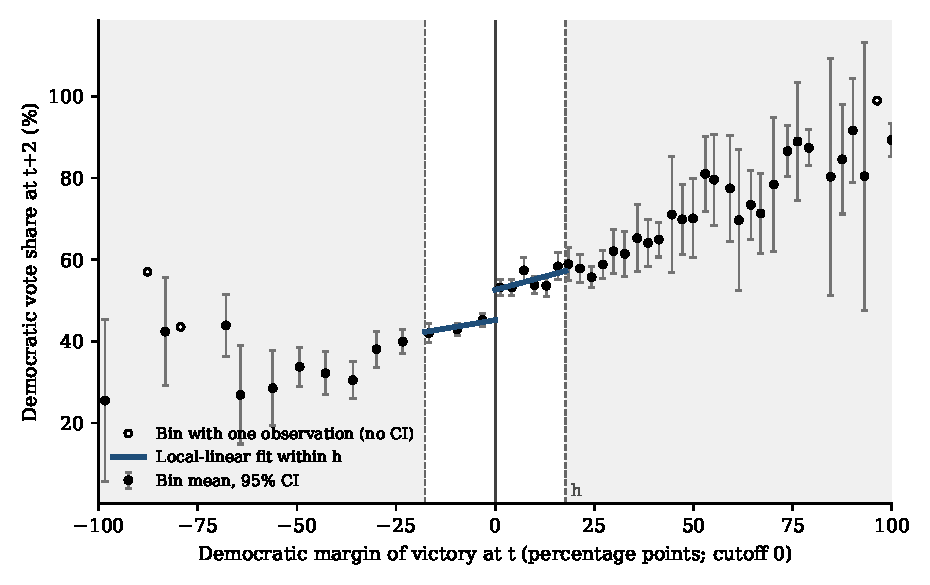
\includegraphics[width=0.85\textwidth]{figures/fig_rd.pdf}
\caption{Democratic vote share at $t+2$ against the Democratic margin at $t$, US Senate elections, 1914--2010, H1 estimation sample. Points are binned means with 95\% intervals. Solid lines are local-linear fits within the MSE-optimal bandwidth $h=\RdBw$ (dashed lines at the cutoff and at $\pm h$). The H1 estimate is \RdEffect\ percentage points, local to close elections. The bandwidth uses \texttt{masspoints = off}, an assumption about the earlier release.}
\label{fig:rd}
\end{figure}

\begin{figure}[t]
\centering
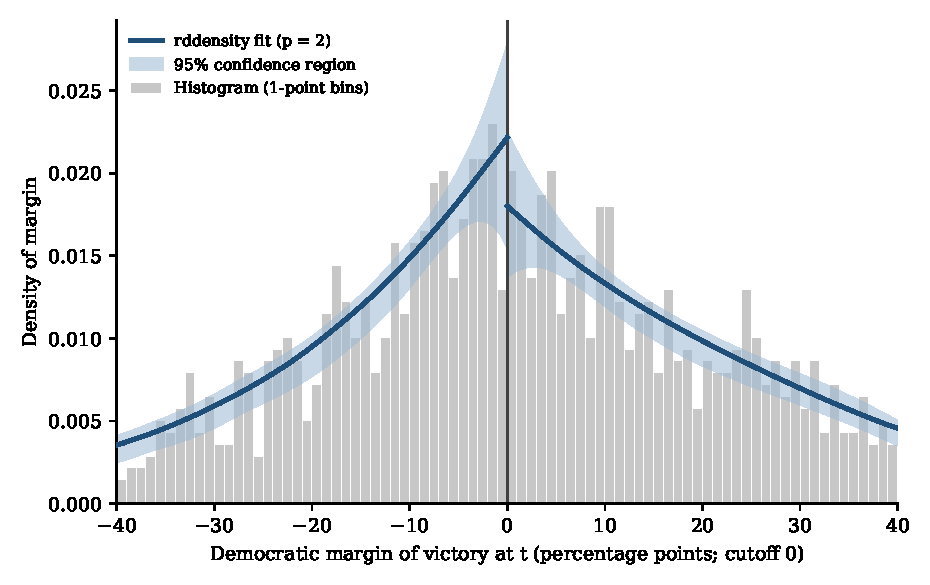
\includegraphics[width=0.85\textwidth]{figures/fig_density.pdf}
\caption{Density of the Democratic margin around the cutoff, all \RdDensityN\ elections (H2(a)). Bars are a histogram in one-point bins over $[-40,40]$. Curves are rddensity local-polynomial estimates on each side with 95\% regions. The robust test gives $T_Q=\RdDensityT$ and $p=\RdDensityP$. The density difference, right minus left, is \RdDensityDiff\ with an MDE of \RdDensityMde. A large p-value is not proof of continuity, and the test has limited power at this sample size.}
\label{fig:density}
\end{figure}

\subsection{Sensitivity to bandwidth and software (H3)}

Panel B of Table~\ref{tab:fals} reports the five descriptive specifications. The printed 2014 bandwidths give an estimate of \RdSensPrintedEst, with a robust interval of $[\RdSensPrintedLo, \RdSensPrintedHi]$. This matches the 2014 interval printed by \citet{calonico2017rdrobust} to the printed precision. Half the H1 bandwidth gives \RdSensHalfEst, double gives \RdSensDoubleEst, and $p=2$ with $q=3$ gives \RdSensPTwoEst. The \texttt{adjust} reading gives \RdSensAdjustEst. Across the five, the point estimate ranges from \RdSensDoubleEst\ to \RdSensHalfEst\ percentage points. Every interval overlaps the H1 interval. The half-bandwidth interval is the widest, running from \RdSensHalfLo\ to \RdSensHalfHi. The sensitivity analysis therefore finds the H1 estimate fairly stable across bandwidths, while the intervals remain wide in the half-bandwidth case. It has no decision rule and is not used to revise the H1 targets.

\section{Limitations}

The estimate is local to close elections, with a bandwidth of about \RdBw\ points, and it is conditional on the Democratic win at the threshold. It does not estimate the incumbency advantage in all Senate elections, and it should not be cited as that estimate.

The falsification tests have low power at this sample size. Each MDE in Table~\ref{tab:fals} is large relative to the quantity it tests, so non-rejection is weak evidence. A density test with an MDE of \RdDensityMde\ cannot show that the running variable is continuous. The covariate and selection tests leave room for effects of the size their MDEs describe. The placebo intervals are wide, and their windows are narrow.

State-clustered inference is not replicated. \citet{calonico2017rdrobust} report a state-clustered variance in Section 7.4, and the paper does not run it. The covariate-adjusted estimates in that section are also not replicated. Both were left out of the approved design, and neither was added after the results were seen.

The primary \texttt{off} setting rests on an unverified assumption about the earlier release. The printed bandwidths discriminate between the two settings, and the \texttt{off} setting reproduces them. The assumption remains unverified.

The file is the CSV from the rdrobust repository, not the \texttt{.dta} used by the authors. The printed descriptive statistics agree, but the outcome's moments were not compared before the H1 run. The estimation software is the Python package at version 2.1.1, not the 2016 Stata release. The reproduction is therefore of the printed numbers under a modern implementation, not of the original code.

The H1 reproduction is a computational check and is not evidence about the incumbency advantage. Its pass is not evidence that the design is right, and a pass under the \texttt{off} setting does not establish that the selection or density assumptions hold.

Finally, two claims in the literature bear on this design, and this paper cannot resolve either. \citet{caughey2011elections} find covariate imbalance in close US House races, which grows in the closest races. \citet{eggers2015validity} argue, from more than 40,000 close races, that the RD assumptions are likely to hold in many electoral settings. Neither paper analyses this Senate file. The Eggers et al. paper was checked against its abstract only.

\section{Deviations from the approved design and disclosures}

The following deviations and disclosures are recorded in \texttt{plan.json} and the run notes. Each is listed here in plain words.
\begin{enumerate}
\item \textbf{Pre-gate computations.} Before the design gate, the data-prep run \texttt{design-mde} computed the robust density test on margin (the H2(a) statistic), the density-difference estimate, its jackknife standard error and the density MDE (\RdDensityMde), and the standard errors of the four covariate tests, which give the H2(b) MDEs. The analysis run \texttt{h2-density} reproduces the statistic and records the MDE as a result claim. It loaded no vote values. The H2(a) result and the H2(b) standard errors were therefore seen before the design gate. The analysis runs repeated these computations with the same settings, and they agree exactly. The PI accepted the pre-gate computations with this disclosure. The Reviewer raised it as a major finding at design-r1 (F4). The PI ruled that the pre-gate computations stand with this disclosure. The Reviewer withdrew the finding at design-r2 and again at design-r3, stating that it was withdrawn on the PI's ruling and that the Reviewer does not override that ruling.
\item \textbf{Printed-value setting.} The H2(b) comparison with the printed p-values is made under both settings. \texttt{off} is primary, consistent with the H1 assumption, and \texttt{adjust} is secondary. The PI first ruled at code-r1 (log 05:31:36Z) that the comparator is \texttt{adjust}, and then at code-r2 (log 05:37:58Z) made \texttt{off} the primary comparison with \texttt{adjust} secondary. Both rulings came before the first analysis run (05:44:27Z). The 0.0005 match rule was set in the code before any analysis run and recorded in the plan disclosures. The design text itself named no setting for this comparison, and the paper states both results.
\item \textbf{Full-file and estimation-sample counts.} The design text quotes counts of distinct margin values and of left and right rows for the full file of \RdDensityN\ rows. The paper uses the counts on the H1 estimation sample of \RdN\ rows, as recorded by \texttt{h1-rdrobust}.
\item \textbf{Post-review metric.} After the results review, the Econometrician added one metric to \texttt{code/h2\_density.py}, the MDE of the density difference (\RdDensityMde). The run \texttt{h2-density} was repeated with \texttt{-{}-replace}. All earlier metrics are unchanged, checked key by key. The superseded run is archived under \texttt{runs/.superseded/}, and the change is logged.
\item \textbf{Mass points in the density test.} rddensity's default \texttt{massPoints = True} is used for H2(a), while H1 uses \texttt{off} for rdrobust. The H1 assumption concerns rdrobust's bandwidth selector, not rddensity. The robust p-value with \texttt{massPoints = False} is reported as a sensitivity check; its value is identical to the main value (Section 4.2).
\item \textbf{Placebo design.} The H2(c) placebos are report-only, with no equivalence bound and no multiplicity correction. The design-stage bound was withdrawn after review, and the placebo cutoffs are computed from margin alone.
\item \textbf{Units of H2(d).} The selection coefficient and interval are on the proportion scale. Section 4.2 converts them to percentage points by a LaTeX calculation from the macros (the pgf package), so no converted number is typed. The MDE is already in percentage points. No percentage-point metric for this test exists in the runs.
\item \textbf{Baseline for H3.} The half and double bandwidths use the printed $b=27.984$ as baseline. The H1 \texttt{off} bias bandwidth is \RdBOff, against the printed 27.984, and the tolerance rule does not test it.
\item \textbf{Clean reruns and tool fixes.} Four clean reruns have been made, each from an environment built from \texttt{code/}\allowbreak\texttt{requirements.txt} alone. The first reproduced 7 of 15 runs. Its failures came from the rerun tool, which omitted \texttt{runs/} from its copy and counted a metric that is NaN in both runs as a mismatch. The PI session fixed the tool (commit \texttt{0a72b72}) and added a test. The NaN rule widens the comparator only for such metrics. The second rerun reproduced 15 of 15 (commit \texttt{c1c9549}), but its \texttt{replication.json} recorded the interpreter that ran \texttt{crew.py} (Python 3.14.6) at the top level. The PI session then changed the tool (commit \texttt{87890ae}) to record each run's interpreter and to label the top-level value \texttt{crew\_python}. The third rerun reproduced 15 of 15, with Python 3.12.11 recorded for every run. The fourth rerun, with \texttt{crew.py} as of its last change (commit \texttt{87890ae}) and the workspace at commit \texttt{a6d7c45}, also reproduced 15 of 15. Its NaN rule covered \texttt{T\_Q\_asy} and \texttt{p\_Q\_asy}, which are NaN in both runs and so are reproduced without being compared. It was needed because the Econometrician reworded two claim texts in \texttt{claims.jsonl} (values unchanged) and reran \texttt{tab-main} and \texttt{tab-falsification} with \texttt{-{}-replace}, which declare \texttt{claims.jsonl} as an input, so the third record was older than those runs. The fourth run's \texttt{replication.json} is the record the submission gate reads. No analysis code, data or tolerance changed. The earlier records are in git history, and \texttt{REPLICATION.md} describes all four runs.

\item \textbf{Post-gate edits and open findings.} The results gate was approved on results-r3, with minor findings F12 to F14 open. Afterwards, without new estimation, the claim texts and NOTES were edited (commit \texttt{48f9767}), and claims for the adjust counts, the H2(d) sample size and the placebo sample sizes were added from runs already recorded. These edits address results-r3 F12 to F14 but were not reviewed before this round. Two minor code-review findings also remain open: the positive branch of the \texttt{bw\_capped} flag is untested on output, which the text states, and the static guard against a read of \texttt{vote} is a substring match, weaker than an exact check. The \texttt{unit-tests} run record also includes a session scratch path in its command, so that command cannot be reproduced from the workspace alone; the run passed on this machine. This is disclosed here and was not changed after review.
\end{enumerate}

\section{Conclusion}

The default output of \citet{calonico2017rdrobust} is reproduced within the tolerance set in advance, under the primary \texttt{off} setting, which is an unverified assumption chosen knowing the printed targets. Under the software default, \texttt{adjust}, the bandwidth and two covariate p-values miss the printed values. The conventional estimate is \RdEffect\ percentage points and the robust interval is $[\RdCiLow, \RdCiHigh]$, on \RdN\ elections. The match is a computational check, and the paper makes no new claim about the incumbency advantage. The estimate is local to close elections.

The falsification checks do not reject, but they are imprecise, and the selection test has a wide interval. This paper gives no link from a change in the observed-outcome share to a bias in the vote estimate. A finding that the design is free of sorting or selection would need more power than this file provides. Across five descriptive sensitivity specifications, the point estimate lies between \RdSensDoubleEst\ and \RdSensHalfEst\ percentage points, which shows how far the printed output moves with the bandwidth and software choices it leaves open.

\section*{AI-use statement}

This paper was drafted by a crew of AI research-assistant agents
(Free-Research-Crew, protocol v0.1) under the direction of the human author, Bryce Wang.
The human approved the research question, the design and the results at three gates.
The submission gate is pending at the time of writing. The human author takes
responsibility for the content.

\begin{itemize}
  \item \textbf{Roles and models.} Every role subagent ran on Claude Haiku 5.5
        (\texttt{claude-haiku-5-5}): Scout, Data RA, Designer, Econometrician, Figures RA,
        Writer and Replicator, and the Reviewer. The PI session ran on Claude Opus 5.5.
  \item \textbf{Review.} The Reviewer agent ran 15 rounds: question (2 rounds, block then
        revise), design (3: revise, revise, pass), code (3: pass, revise, pass), results
        (3: revise, revise, pass) and paper (4: revise, revise, revise, revise). Every round
        was fresh-context. The Reviewer ran on the same model family as the authoring agents,
        so the independence level is fresh-context, not cross-family. The paper stage has been
        reviewed four times, and none of the four rounds passed. The reviews and the
        Reviewer's memory are in \texttt{reviews/}.
  \item \textbf{Findings accepted over the Reviewer: one.} design-r1 F4 (pre-gate
        computations in \texttt{design-mde}), kept by the PI's ruling with a disclosure,
        withdrawn by the Reviewer at design-r2 and design-r3, and shown to the human at the
        design gate.
  \item \textbf{Open findings at the question gate.} The human approved the question gate at
        04:22:30Z, with question-r2 F4, F7 and F8 deferred to the design stage, and question-r2
        F9 answered by the PI. The question stage was not re-reviewed after that, so those four
        records still read open. The design stage addressed their substance: the MDEs and the
        non-rejection wording (F4), the data checks (F7), a data check (F8), and the one-sided
        placebo cutoffs (F9). F8 is only partly met. The CSV's non-outcome moments match
        CCFT's printed values, but the CSV is not the \texttt{.dta} file CCFT used, and the
        moments of \texttt{vote} were not compared before the H1 run.
  \item \textbf{Clean reruns.} Four clean reruns, each from an environment built from
        \texttt{code/}\allowbreak\texttt{requirements.txt} alone. The first reproduced 7 of 15
        runs; its failures came from the rerun tool (it omitted \texttt{runs/} and counted a NaN
        in both runs as a mismatch), and the PI session fixed the tool (commit
        \texttt{0a72b72}). The second reproduced 15 of 15 (commit \texttt{c1c9549}), but its
        \texttt{replication.json} recorded the tool's interpreter at the top level. The PI
        session then changed the tool (commit \texttt{87890ae}) to record each run's interpreter
        and label the top-level value \texttt{crew\_python}. The third reproduced 15 of 15 with
        Python 3.12.11 recorded for every run. The fourth reproduced 15 of 15, with
        \texttt{crew.py} as of its last change (commit \texttt{87890ae}) and the workspace at
        commit \texttt{a6d7c45}. It was rerun because two claim texts were reworded (values
        unchanged) and two tables were regenerated, which made the third record older than its
        inputs. The NaN rule covered two metrics, \texttt{T\_Q\_asy} and \texttt{p\_Q\_asy}, which
        are NaN in both runs and so are reproduced without being compared. The fourth run's
        \texttt{replication.json} is the record the submission gate reads. No analysis code,
        data or tolerance changed. \texttt{REPLICATION.md} describes all four runs.
  \item \textbf{Briefs.} The role briefs are archived in \texttt{briefs/}.
  \item \textbf{Evidence.} Every reported number is generated from a logged run through
        the macro file \texttt{numbers.tex}. Every citation was checked against its source:
        four from the full text, and Eggers et al. (2015) from its abstract only. The full
        text of Cattaneo, Frandsen and Titiunik (2015) was read from a third-party mirror on
        GitHub (nbviewer). Its printed title, authors and DOI match the publisher record,
        and \texttt{sources/sources.json} records the DOI. The full workspace is
        \texttt{gallery/ss-rd-senate} in the Auto-Research-Skills repository; the public URL
        is to be added at release.
\end{itemize}


\bibliographystyle{plainnat}
\bibliography{../refs}

\end{document}
